\documentclass[11pt]{article}

% ---------- Packages (per course conventions) ----------
\usepackage[margin=1in]{geometry}
\usepackage{graphicx}
\usepackage{float}
\usepackage{booktabs}
\usepackage{siunitx}
\usepackage{amsmath}
\usepackage{amssymb}
\usepackage{tikz}
\usepackage{enumitem}
\usepackage{xcolor}
\usepackage{caption}
\PassOptionsToPackage{hyphens}{url}
\usepackage{hyperref}
\hypersetup{colorlinks=true, linkcolor=black, citecolor=black, urlcolor=blue}


\setlength{\parindent}{0pt}
\setlength{\parskip}{0.6\baselineskip}
\setlist{nosep, leftmargin=1.5em}
\captionsetup{font=small, skip=4pt}
\sisetup{group-separator={,}, group-minimum-digits=4}

\begin{document}

% =========================================================
% COVERSHEET
% =========================================================
\begin{titlepage}
    \centering
    \vspace*{2cm}
    {\LARGE \bfseries ENGR 225: Mechanics 1} \\[0.3cm]
    {\Large Homework Coversheet} \\[0.3cm]
    {\large Assoc.\ Prof.\ Clayton Byers} \\[2cm]

    \begin{flushleft}
        \Large
        \textbf{NAME:} \underline{\makebox[10cm][l]{\ Sean Balbale}} \\[1cm]
        \textbf{DATE:} \underline{\makebox[10cm][l]{\ 6 November 2026}} \\[1cm]
        \textbf{ASSIGNMENT:} \underline{\makebox[9cm][l]{\ Design Project, Part 1}} \\[2cm]
    \end{flushleft}

    \large
    \textbf{Level of involvement of AI, LLMs, or related tools in the completion of this assignment:}

    \vspace{1cm}

    \begin{flushleft}
        \Large
        $\square$ \quad None \\[0.7cm]
        $\square$ \quad Minor \\[0.7cm]
        $\blacksquare$ \quad Major \\[0.7cm]
        $\square$ \quad Extensive \\[1.5cm]
    \end{flushleft}

    \normalsize
    \textit{Mark the box that applies (e.g., replace $\square$ with $\blacksquare$, or type an X beside it, before compiling/printing). Your disclosure does not affect your grade -- it keeps you accountable for the work you are doing.}
\end{titlepage}

% =========================================================
% REPORT
% =========================================================
\begin{center}
    {\Large \bfseries ENGR 225 Design Project, Part 1: Roadway Selection} \\[0.2cm]
    Sean Balbale \hfill Assigned: 26 Oct 2026 \hfill Due: 6 Nov 2026
\end{center}

\section{Objective}
The objective of Part~1 is to select and quantify the roadway that the truss bridge will carry. The specific goals are:
\begin{itemize}
    \item To classify the roadway and select lane, shoulder, and barrier widths from AASHTO and CTDOT standards.
    \item To specify the deck section (slab, waterproofing, wearing surface) and calculate material quantities for the \SI{60}{m} span.
    \item To estimate the cradle-to-gate embodied carbon of those materials and compare it against lower-carbon alternatives.
    \item To estimate the raw material cost.
\end{itemize}

\section{Design Basis}
\paragraph{Given Parameters}
\begin{itemize}
    \item \textbf{Span:} $L = \SI{60}{m}$, two lanes per direction, no pedestrian traffic.
    \item \textbf{Reference roadway:} Route~2 over Griswold St., Glastonbury: \num{74400} vehicles/day, 6\% trucks (2021) \cite{nbi_griswold}, or about \num{4460} trucks/day.
    \item \textbf{Classification:} urban principal arterial freeway (divided, full access control).
    \item \textbf{Standards:} AASHTO freeway criteria for widths \cite{fhwa_pts}; CTDOT Bridge Design Manual and pavement guidance for the deck section \cite{ctdot_bdm8, ctdot_overlay}.
\end{itemize}

\section{Roadway Design}

\paragraph{Cross-Section}
AASHTO sets a \SI{12}{ft} minimum lane width and a \SI{10}{ft} minimum shoulder, except that the left shoulder of a 4-lane freeway can be \SI{4}{ft} \cite{fhwa_pts}. I used the minimums, since every foot of width carries into the slab, rebar, and overlay quantities. The bridge carries the full approach width. Each edge has a \SI{32}{in} concrete parapet and the median has a \SI{42}{in} barrier; the barrier base widths (\SI{21}{in} and \SI{24}{in}) are my assumptions, not CTDOT plate values.

\begin{figure}[H]
\centering
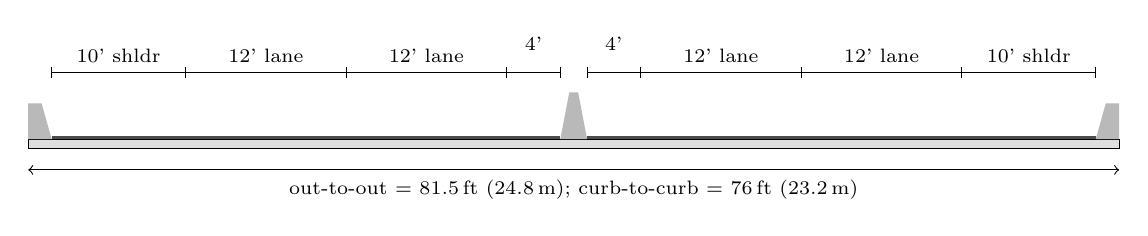
\begin{tikzpicture}[x=0.17cm, y=0.17cm, font=\scriptsize]
    \fill[gray!25] (0,0) rectangle (81.5,-0.71);
    \draw (0,0) rectangle (81.5,-0.71);
    \fill[black!70] (1.75,0) rectangle (39.75,0.25);
    \fill[black!70] (41.75,0) rectangle (79.75,0.25);
    \fill[gray!55] (0,0) -- (1.75,0) -- (1.0,2.67) -- (0,2.67) -- cycle;
    \fill[gray!55] (81.5,0) -- (79.75,0) -- (80.5,2.67) -- (81.5,2.67) -- cycle;
    \fill[gray!55] (39.75,0) -- (41.75,0) -- (41.08,3.5) -- (40.42,3.5) -- cycle;
    \foreach \x in {1.75,11.75,23.75,35.75,39.75,41.75,45.75,57.75,69.75,79.75}
        \draw (\x,4.6) -- (\x,5.4);
    \draw (1.75,5) -- (39.75,5); \draw (41.75,5) -- (79.75,5);
    \node[above] at (6.75,5) {10' shldr};
    \node[above] at (17.75,5) {12' lane};
    \node[above] at (29.75,5) {12' lane};
    \node[above] at (37.75,5.9) {4'};
    \node[above] at (43.75,5.9) {4'};
    \node[above] at (51.75,5) {12' lane};
    \node[above] at (63.75,5) {12' lane};
    \node[above] at (74.75,5) {10' shldr};
    \draw[<->] (0,-2.3) -- (81.5,-2.3) node[midway, below] {out-to-out = \SI{81.5}{ft} (\SI{24.8}{m}); curb-to-curb = \SI{76}{ft} (\SI{23.2}{m})};
\end{tikzpicture}
\caption{Roadway cross-section: \SI{3}{in} HMA on membrane over an \SI{8.5}{in} reinforced concrete slab (vertical not to scale).}
\label{fig:section}
\end{figure}

\paragraph{Deck Section}
\begin{itemize}
    \item \textbf{Slab:} \SI{8.5}{in} (\SI{216}{mm}) cast-in-place reinforced concrete, the CTDOT minimum, with \SI{2.5}{in} cover over the top mat \cite{ctdot_bdm8}. Reinforcement is assumed at \SI{150}{kg/m^3} until Part~2 sizes it.
    \item \textbf{Waterproofing:} spray-applied liquid membrane, CTDOT's current standard under a bituminous surface \cite{ctdot_overlay}.
    \item \textbf{Wearing surface:} \SI{3}{in} hot-mix asphalt (HMA): a \SI{1}{in} S0.25 lift on the membrane and a \SI{2}{in} top course \cite{ctdot_overlay}.
\end{itemize}

\paragraph{Quantities}
With out-to-out width $W = \SI{24.84}{m}$ and curb-to-curb width $w_c = \SI{23.16}{m}$:
\begin{align*}
V_{\text{deck}} &= L W t_s = (\SI{60}{m})(\SI{24.84}{m})(\SI{0.216}{m}) = \SI{322}{m^3} \\
V_{\text{barrier}} &= L(2A_p + A_m) = (\SI{60}{m})(2 \times \SI{0.279}{m^2} + \SI{0.434}{m^2}) = \SI{59.5}{m^3} \\
m_{\text{rebar}} &= (\SI{381}{m^3})(\SI{150}{kg/m^3}) = \SI{57.2}{t} \\
m_{\text{HMA}} &= L w_c t_o \rho_{\text{HMA}} = (\SI{60}{m})(\SI{23.16}{m})(\SI{0.0762}{m})(\SI{2.35}{t/m^3}) = \SI{249}{t}
\end{align*}
Total concrete is \SI{381}{m^3} (\SI{499}{yd^3}).

\section{Environmental Impact}

\paragraph{Embodied Carbon}
I used environmental product declarations (EPDs), which report cradle-to-gate (A1--A3) CO$_2$e per unit of material. A Connecticut-area \SI{4000}{psi} EPD covers mixes from \SIrange{265}{335}{kg/m^3} \cite{epd_conco}, so I used the \SI{300}{kg/m^3} midpoint. Rebar is \SI{854}{kg/t} from the CRSI industry average \cite{crsi_epd}, and HMA is \SI{71.1}{kg/t} from an FHWA example EPD \cite{fhwa_edc7}.

\begin{table}[H]
    \centering
    \caption{Baseline embodied carbon (A1--A3)}
    \label{tab:carbon}
    \begin{tabular}{lccc}
        \toprule
        \textbf{Material} & \textbf{Quantity} & \textbf{GWP Factor} & \textbf{CO$_2$e (t)} \\
        \midrule
        Concrete (deck + barriers) & \SI{381}{m^3} & \SI{300}{kg/m^3} & 114 \\
        Reinforcing steel & \SI{57.2}{t} & \SI{854}{kg/t} & 48.8 \\
        HMA overlay & \SI{249}{t} & \SI{71.1}{kg/t} & 17.7 \\
        \midrule
        \textbf{Total} & & & \textbf{181} \\
        \bottomrule
    \end{tabular}
\end{table}

Concrete is 63\% of the total, and nearly all of that is the portland cement, which emits CO$_2$ from both kiln fuel and limestone calcination. The membrane is excluded since I could not find an EPD for it; it is a few millimeters thick, so its mass is small next to the slab.

\paragraph{Alternatives}
\begin{table}[H]
    \centering
    \caption{Embodied carbon of alternative materials (same geometry)}
    \label{tab:alts}
    \begin{tabular}{lcc}
        \toprule
        \textbf{Option} & \textbf{CO$_2$e (t)} & \textbf{Change} \\
        \midrule
        Baseline & 181 & -- \\
        Slag-cement concrete, 40--50\% lower GWP \cite{pulse_scm} & 124--135 & $-25$ to $-32\%$ \\
        EAF rebar on renewable power, \SI{300}{kg/t} \cite{epd_xcarb} & 149 & $-18\%$ \\
        Concrete wearing surface instead of HMA & 195 & $+8\%$ \\
        Slag concrete (45\%) + EAF rebar & 98 & $-46\%$ \\
        \bottomrule
    \end{tabular}
\end{table}

Cement content is the biggest lever: a 60\% slag mix approved for Australian infrastructure cut embodied carbon by an estimated 40--50\% \cite{pulse_scm}, at the cost of slower early strength gain. HMA is also the better wearing surface on carbon, not just by CTDOT practice; replacing it with \SI{106}{m^3} of concrete adds \SI{14}{t}.

\paragraph{Perspective}
EPA puts a typical passenger vehicle at about \SI{400}{g} CO$_2$ per mile \cite{epa_vehicle}, so traffic over the span emits
\[
(\num{74400}/\text{day})\left(\frac{\SI{60}{m}}{\SI{1609}{m/mi}}\right)(\SI{0.400}{kg/mi}) = \SI{1.11}{t/day}.
\]
The baseline materials equal about 163 days of that traffic. This slightly overstates the ratio since trucks emit more per mile than cars, but the materials are the part of the footprint the designer controls.

\paragraph{Other Impacts}
The concrete and HMA contain several hundred tonnes of quarried aggregate, with the land disturbance and truck traffic that comes with it. The A1--A3 figures also stop at the plant gate, so a distant plant with a lower EPD value can come out worse once hauling is counted. Recycled asphalt pavement (RAP) in the HMA cuts virgin aggregate and binder demand.

\section{Raw Material Cost}

\begin{table}[H]
    \centering
    \caption{Raw material cost (2026 USD, excluding labor and formwork)}
    \label{tab:cost}
    \begin{tabular}{lccc}
        \toprule
        \textbf{Material} & \textbf{Quantity} & \textbf{Unit Price} & \textbf{Cost} \\
        \midrule
        Ready-mix concrete & \SI{499}{yd^3} & \$185/yd$^3$ \cite{concrete_ne} & \$92{,}200 \\
        Reinforcing steel & \SI{57.2}{t} & \$1{,}100/t \cite{gmk_rebar} & \$62{,}900 \\
        HMA & \SI{274}{short~tons} & \$130/ton \cite{ctdot_bid_0155} & \$35{,}700 \\
        \midrule
        \textbf{Total} & & & \textbf{\$191{,}000} \\
        \bottomrule
    \end{tabular}
\end{table}

Concrete is priced at the top of the \$155--\$185/yd$^3$ Northeast range \cite{concrete_ne}, since a deck mix is air-entrained and higher strength than residential concrete. Rebar rounds up from the \$1{,}058/t US average at the start of 2026 \cite{gmk_rebar} to cover fabrication. HMA is a CTDOT bid price for S0.5 (\$129--\$135/ton) \cite{ctdot_bid_0155}, which includes placement, so it is an upper bound. The same contract bid deck concrete at \$700--\$915/yd$^3$ installed, so raw concrete is only 20--26\% of the in-place cost.

\section{Conclusion}
The roadway is a 4-lane urban freeway deck, \SI{60}{m} long and \SI{24.8}{m} wide out-to-out.
\begin{enumerate}
    \item \textbf{Geometry:} four \SI{12}{ft} lanes, \SI{10}{ft} right and \SI{4}{ft} left shoulders, \SI{76}{ft} curb-to-curb. Widening the left shoulders to \SI{10}{ft} would add about 15\% to the deck and overlay quantities.
    \item \textbf{Deck section:} \SI{8.5}{in} reinforced concrete slab, liquid membrane, and \SI{3}{in} HMA, giving \SI{381}{m^3} of concrete, \SI{57.2}{t} of rebar, and \SI{249}{t} of HMA.
    \item \textbf{Embodied carbon:} \SI{181}{t} CO$_2$e, 63\% from concrete. Slag cement and EAF rebar together bring it to about \SI{98}{t} ($-46\%$).
    \item \textbf{Cost:} about \$191{,}000 in raw materials, 48\% of it concrete.
\end{enumerate}
Slab thickness and rebar density are the values most likely to change once Part~2 sizes the truss and the deck span between supports.

\paragraph{AI Use}
I used Claude (Anthropic) to locate the CTDOT, FHWA, and EPD sources, check the quantity and carbon arithmetic, and draft and edit this report. I checked each design value against its cited source and made the classification, shoulder-width, and material decisions myself.

% =========================================================
% BIBLIOGRAPHY (IEEE)
% =========================================================
\begin{thebibliography}{99}
\footnotesize
\setlength{\itemsep}{0pt}

\bibitem{nbi_griswold}
``Route 2 over Griswold Street, Glastonbury, CT,'' National Bridge Inventory record, BridgeLookup. [Online]. Available: \url{https://bridgelookup.com/bridge/74712}

\bibitem{fhwa_pts}
Federal Highway Administration, ``Chapter 8: Geometric design,'' in \emph{Use of Freeway Shoulders for Travel}, FHWA-HOP-15-023. [Online]. Available: \url{https://ops.fhwa.dot.gov/Publications/fhwahop15023/ch8.htm}

\bibitem{ctdot_bdm8}
Connecticut Department of Transportation, ``Section 8: Decks and deck protective systems,'' in \emph{Bridge Design Manual}, Newington, CT, USA. [Online]. Available: \url{https://portal.ct.gov/-/media/DOT/documents/dpublications/bridge/Division-1/Section-08-Decks-and-Deck-Protective-Systems.pdf}

\bibitem{ctdot_overlay}
Connecticut Department of Transportation, Pavement Design Unit, ``Bridge deck overlay guidance,'' Dec. 14, 2022. [Online]. Available: \url{https://portal.ct.gov/-/media/dot/documents/dpavement/bridge_deck_overlay_guidance_12-14-22.pdf}

\bibitem{epd_conco}
Conco Companies, Sherman St. Plant, ``Ready-mix concrete, 4000 psi,'' NRMCA EPD 20142, 2025, via One Click LCA. [Online]. Available: \url{https://materials.oneclicklca.com/it/material/ready-mix-concrete/68e016f78c603d767267f93e}

\bibitem{crsi_epd}
Concrete Reinforcing Steel Institute, ``Environmental product declaration: Fabricated steel reinforcement,'' ASTM International EPD 362. [Online]. Available: \url{https://www.crsi.org/sustainability/environmental-product-declaration/}

\bibitem{fhwa_edc7}
Federal Highway Administration, ``Environmental product declarations,'' Every Day Counts (EDC-7) fact sheet. [Online]. Available: \url{https://www.fhwa.dot.gov/innovation/everydaycounts/edc_7/docs/EDC-7FactsheetEPDs.pdf}

\bibitem{pulse_scm}
``Advancing low carbon concrete in Australian infrastructure,'' \emph{Roads \& Infrastructure Australia}, Apr. 1, 2026. [Online]. Available: \url{https://www.pulse.bot/construction/news/advancing-low-carbon-concrete-in-australian-infrastructure-31d0c281-fa9e-4b83-b868-9dd11e86ee4a}

\bibitem{epd_xcarb}
ArcelorMittal Europe, ``XCarb recycled and renewably produced reinforcing steel,'' EPD, via One Click LCA. [Online]. Available: \url{https://materials.oneclicklca.com/en/material/reinforcing-steel-rebar/63186018eacb8327acb30d11}

\bibitem{epa_vehicle}
U.S. Environmental Protection Agency, ``Greenhouse gas emissions from a typical passenger vehicle,'' EPA-420-F-23-014, Jun. 2023. [Online]. Available: \url{https://www.epa.gov/greenvehicles/greenhouse-gas-emissions-typical-passenger-vehicle}

\bibitem{concrete_ne}
``Average concrete cost by state in 2026,'' UseCalcPro. [Online]. Available: \url{https://usecalcpro.com/blog/average-concrete-cost-by-state-2026}

\bibitem{gmk_rebar}
GMK Center, ``Prices for rebar showed mixed dynamics at the beginning of the year,'' 2026. [Online]. Available: \url{https://gmk.center/en/news/prices-for-rebar-showed-mixed-dynamics-at-the-beginning-of-the-year/}

\bibitem{ctdot_bid_0155}
Connecticut Department of Transportation, ``Tabulation of bids, State Project 0155-0169.'' [Online]. Available: \url{https://portal.ct.gov/-/media/dot/documents/dcontracts/01550169bidtabspdf.pdf}

\end{thebibliography}

\end{document}